\chapter{Bayesian Modeling of Multi-player Games}
\chaptertoc

%%% Nothing in Nature is random. ... A thing appears random only through the incompleteness of our knowledge.
%%% - Benedict Spinoza -

\begin{quotation}\textit{
On voit, par cet Essai, que la théorie des probabilités n'est, au fond, que le bon sens réduit au calcul; elle fait apprécier avec exactitude ce que les esprits justes sentent par une sorte d'instinct, sans qu'ils puissent souvent s'en rendre compte.
\vspace{0.2cm} \\
One sees, from this Essay, that the theory of probabilities is basically just common sense reduced to calculus; it makes one appreciate with exactness that which accurate minds feel with a sort of instinct, often without being able to account for it.}
\begin{flushright}Pierre-Simon Laplace (1814)\end{flushright}\end{quotation}

\lettrine{H}{ere}, we now present the use of probability theory as an alternative to logic, transforming incompleteness into uncertainty. Bayesian models can deal with both intentional and extensional uncertainty, that is: uncertainty coming from intentions of the players or the stochasticity of the game, as well as uncertainty coming from imperfect information and the model's limits. We will first show how these problems are addressed by probabilities and how to structure a full Bayesian program. We illustrate the approach with a model evaluated on a simulated \glos{MMORPG} situation.

%Bot AI has to be adaptive, robust, multi-scale.
%Why?
%\begin{itemize}
%\item The bot can't cheat (at least it's not fun!)
%\item The bot can't assume optimal play from the opponent when the problem is so large
%\item The bot can learn from others games, self past games, self current game
%\item The bot can't be in the head of your opponent (meta-)
%\end{itemize}

\section{Characteristics of Game AI}

\subsection{Partial information}
If the AI has perfect information, behaving realistically is the problem. Cheating bots are not fun, so either AI should just use information available to the players, or it should fake having only partial information. In probabilistic modeling, sensor models allow for the computation of the state $S$ from observations $O$ by asking $\PP(S|O)$. One can easily specify or learn $\PP(O|S)$: either the game designers specify it, or the bot uses perfect information to get $S$ and leanrs (counts) $\PP(O|S)$. Then infer $\PP(S|O) = \frac{\PP(O|S).\PP(S)}{\PP(O)}$ (Bayes rule). Incompleteness of information is just uncertainty about the full state.

\subsection{Randomness}
Some games have inherent stochasticity (variable random action effects) part of the gameplay, and even for other games, an AI can't assume optimal play from the opponent. In the context of state estimation and control, dealing with this randomness require ad-hoc methods for scripting of boolean logic, while it is dealt with natively with probabilistic models. Where a program would have to test for the action effect/value $V$ to be in a given interval to decide on a given course of action $A$, a probabilistic models just computes $\PP(A|E) = \frac{\PP(E|A).\PP(A)}{\PP(E)}$.

\subsection{Vertical continuity}
Abstracting higher level cognitive functions (strategy and tactics for instance) is an efficient way to break the complexity barrier of writing game AI. Exploiting the vertical continuity, i.e. the conditioning of higher level thinking on actions, is totally possible in a hierarchical Bayesian model. With strategies as values of $S$ and tactics as values of $T$, $\PP(T|S)$ gives the conditioning of $T$ on $S$ and thus enables us to evaluate only those $T$ values that are possible with given $S$ values.

\subsection{Horizontal continuity}
Real-time games may use discrete time-steps (24Hz for instance for StarCraft), it does not prevent temporal continuity in strategies, tactics and, most strongly, actions. There are several Bayesian models able to deal with sequences, filter models, from which \newglossaryentry{HMM}{name=HMM,description={Hidden Markov Model, a dynamic Bayesian network estimating hidden states following a Markov process from observations}}Hidden Markov Models (\glos{HMM}) \citep{Rabiner}, Kalman filters \citep{Kalman1960} and particle filters \citep{particleFiltering} are specializations of. With states $S$ and observations $O$, filter models under the Markov assumption represent the joint $\PP(S^0).\PP(O^0|S^0).\prod_{t=1}^T[\PP(S^t | S^{t-1}).\PP(O^t|S^t)]$.

\subsection{Autonomy and Programming}
Autonomy is the ability to deal with new states, the challenge of autonomous characters arises from state spaces too big to be fully specified (in scripts / FSM). Again, probabilistic modeling enables one to recognize unspecified states as soft mixtures of known states, of deal with unknown state as an incomplete version of a known state which subsumes it. Autonomy can also be reached through learning, being it through online or offline learning. Offline learning is used to learn parameters that does not have to be specified by the programmers and/or game designers. One can use data or experiments with known/wanted situations (supervised learning, reinforcement learning), or explore data (unsupervised learning) or game states (evolutionary algorithms). Online learning can provide adaptivity of the AI to the player and/or its own competency playing the game.

\section{The Bayesian Programming Methodology}
The reverend Thomas Bayes is the first credited to have worked on inversing probabilities: by knowing something about the probability of $A$ given $B$, how can one draw conclusions on the probability of $B$ given $A$? Bayes theorem states: $$\PP(A|B) = \frac{\PP(B|A)P(A)}{\PP(B)}$$
\cite{Laplace} rediscovered this theorem and published the work of inductive reasoning by using probabilities. Later, by extending logic to \textit{plausible reasoning}, \cite{Jaynes} arrived at the same properties than \cite{Kolmogorov33} probability theory. Plausible reasoning originates from logic, whose statements have degrees of plausibility represented by real numbers. %We note ``the conditional plausibility that A is true, given that B is true'' $A|B$.
Adding consistency: a) all the possible ways to reach a conclusion leads to the same result, b) information cannot be ignored, c) two equal states of knowledge have the same plausibilities; Jaynes derived the ``product-rule'' ($\PP(AB)=\PP(A\cap B)=\PP(A|B)\PP(B)$) and the ``sum-rule'' ($\PP(A+B)=\PP(A)+\PP(B)-\PP(AB)$ or $\PP(A\cup B) = \PP(A)+\PP(B)-\PP(A\cap B)$) of probabilities. As for rules of inferences, the links between logic and plausible reasoning are direct, with $C=[A\Rightarrow B]$:
\begin{itemize}
    \item modus ponens $$\frac{[A\Rightarrow B] \wedge [A=true]}{B=true}$$ translates to $$\PP(B|AC)=\frac{\PP(AB|C)}{\PP(A|C)}$$
    \item modus tollens $$\frac{[A\Rightarrow B] \wedge [B=false]}{A=false}$$ translates to $$\PP(A|C\neg B)=\frac{\PP(A \neg B|C)}{\PP(\neg B|C)}$$
\end{itemize}
Also, additionally to the two strong logic syllogisms above, plausible reasoning gets two weak syllogisms, from:
\begin{itemize}
    \item $$\PP(A|BC)=\PP(A|C)\frac{\PP(B|AC)}{\PP(B|C)}$$ we get $$\frac{[A\Rightarrow B] \wedge [B=true]}{A\ \mathrm{becomes\ more\ plausible}}$$
    \item $$\PP(B| C\neg A)=\PP(B|C)\frac{\PP(\neg A|BC)}{\PP(\neg A|C)}$$ we get $$\frac{[A\Rightarrow B] \wedge [A=false]}{B\ \mathrm{becomes\ less\ plausible}}$$
\end{itemize}

Indeed, this was proved by \cite{Cox46}, producing Cox's theorem (also named Cox-Jayne's theorem):
\begin{mythm}
A system for reasoning which satisfies:
\begin{itemize}
    \item divisibility and comparability, the plausibility of a statement is a real number,
    \item common sense, in presence of total information, reasoning is isomorphic to Boolean logic,
    \item consistency, two identical mental states should have the same degress of plausibility,
\end{itemize}
is isomorphic to probability theory.
\end{mythm}
So the degrees of belief,of any consistent induction mechanism, verify Kolmogorov's axioms. \cite{DeFinetti37} showed that if reasoning is made in a system which is not isomorphic to probability theory, then it is always possible to find a \textit{Dutch book} (a set of bets which guarantees a profit regardless of the outcomes).


Inspired by plausible reasoning, we present Bayesian programming, a formalism that can be used to describe entirely any kind of Bayesian model. It subsumes Bayesian networks and Bayesian maps, as it is equivalent to probabilistic factor graphs \cite{Diard03}. There are mainly two parts in a \newacronym{BP}{BP}{Bayesian program}\glos{BP}, the \textbf{description} of how to compute the joint distribution, and the \textbf{question(s)} that it will be asked. 

The description consists in exhibiting the relevant \textit{variables} $\{X^1,\dots,X^n\}$ and explain their dependencies by \textit{decomposing} the joint distribution $\PP(X^1\dots X^n | \delta, \pi)$ with existing preliminary (\textit{prior}) knowledge $\pi$ and data $\delta$. The \textit{forms} of each term of the product specify how to compute their distributions: either parametric forms (laws or probability tables, with free parameters that can be learned from data $\delta$) or recursive questions to other Bayesian programs.

Answering a question is computing the distribution $\PP(Searched | Known)$, with $Searched$ and $Known$ two disjoint subsets of the variables. 
%%%$P(Searched | Known) = \begin{small} \frac{\sum_{Free}P(Searched\ Free\ Known)}{P(Known)} \end{small} = \frac{1}{Z}\times \sum_{Free} P(Searched\ Free\ Known)$. 
\begin{eqnarray}
& & \PP(Searched | Known) \\
& = & \frac{\sum_{Free}\PP(Searched,\ Free,\ Known)}{\PP(Known)} \\
& = & \frac{1}{Z}\times \sum_{Free} \PP(Searched,\ Free,\ Known)
\end{eqnarray}

General Bayesian inference is practically intractable, but conditional independence hypotheses and constraints (stated in the description) often simplify the model. Also, there are different well-known approximation techniques, for instance Monte Carlo methods \cite{MacKay} and variational Bayes \cite{Beal}.

\begin{small}
\begin{eqnarray*}
BP
\begin{cases}
Desc.
    \begin{cases}
    Spec. (\pi)
        \begin{cases}
        Variables\\
        Decomposition\\
        Forms\ (Parametric\ or\ Program)
        \end{cases}\\
    Identification\ (based\ on\ \delta)
    \end{cases}\\
Question
\end{cases}
\end{eqnarray*}
\end{small}


For the use of Bayesian programming in sensory-motor systems, see \cite{PRDMSMS}. For its use in cognitive modeling, see \cite{Colas10}. For its first use in video games (first person shooter gameplay, Unreal Tournament), see \cite{LeHy04}. \$\$\$


To sum-up, by viewing probabilities as an extension of logic, the method by which to build Bayesian models gets clearer: there is a strong parallel between writing a Bayesian program and logic or declarative programming. In order:
\begin{enumerate}
    \item Isolate the variables of the problem: it is the first prior that the programmer puts into the system. The variables can be anything, from existing input or output values of the problem to abstract/aggregative values or parameters of the model. Discovering which variable to use for a given problem is one of the most complicated form of machine learning.
    \item Suppose and describe the influences and dependencies between these variables. This is another prior that the programmer can have on the problem, and learning the structure between these variables is the second most complicated form of learning.
    \item Fill the priors and conditional probabilities parameters. The programmer needs to be an expert of the problem to put relevant parameters, although this is the easiest to learn from data once variables and structure are specified. Learning the structure can be seen as learning the parameters of a fully connected model (and then removing dependencies where are the less influent parameters) but most of these kinds of model are totally untractable.
\end{enumerate}
In the following, we will show this method applied to a simulated \glos{MMORPG} fight situation.


%%% How?
%%% \begin{itemize}
%%% \item Bayesian programming methodology
%%% \item When in doubt, toss the distribution to your neighbour
%%% \item Exploit gameplay/game rules structure
%%% \item Learn and eat data for breakfast
%%% \item Meta- can be solved by being (globally) stateless and applying the same model as self on the opponent with her sensory inputs
%%% \end{itemize}

\section{Modeling of a Bayesian MMORPG player}

We will now present a model of a MMORPG player with the Bayesian programming framework \citep{SYNNAEVE:MMORPG}. It deals only with a sub-task of a global AI for autonomous NPC. The problem that we try to solve is: how do we choose which skill to use and on which target in a PvE battle? Possible targets are all our allies and foes. Possible skills are all that we know, we will just try and get a distribution over target and skills and pick the most probable combination that is yet possible to achieve (enough energy/mana, no cooldown). For that, we first choose what should be the target given all surrounding variables: is an ally near death that he should be healed, which foe should we focus our attacks on? Once we have the distribution over possible targets, we search the distribution about our skills, pondered by the one on targets. We put extra care in having the same input variables as a human player to keep consistent with our goal of modeling a human. However, some variables can be things that humans subconsciously interpolate from perceptions.

\subsection{Variables}

A very simple set of variables is as follows. We have the $n$ characters as possible targets; each of them has a lot of bound variables. Health/Hit points ($HP$) are discretized in 10 levels, from the lower to the higher. Distance ($D$) is discretized in 4 zones around the robot character: contact where it can attack with a contact weapon and then to the further for which we have to move even for shooting the longest distance weapon/spell. Ally ($A$) is a Boolean variable mentioning if character $i$ is allied with the robot character. Delta hit points ($\Delta HP$) is a 3-valued interpolated value from the previous few seconds of fight that informs about the $i$th character getting wounded or healed (or nothing). Imminent death ($ID$) is also an interpolated value that encodes $HP$, $\Delta HP$ and incoming attacks/attackers. This is a Boolean variable saying if the $i$th character if going to die anytime soon. This is an example of what we consider that an experienced human player will infer automatically from the screen and notifications. Class ($C$), simplified over 4 values, gives the type of the $i$th character: a Tank can take a lot of damages and taunt enemies, a Contact damager can deal huge amounts of damage with contact weapons (rogue, barbarian...), Ranged stands for the class that deals damages from far away (hunters, mages...) and Healers are classes that can heal (in considerable amounts). The Resist variable is the combination of binary variables of resistance to certain types of (magical) damages into one variable. With 3 possible resistances we get ($2^3$) 8 possible values. For instance ``$R_i=FireNat$'' means that the $i$th character resists fire and nature-based damages. Armor (physical damages) could have been included, and the variables could have been separated. The skill variable takes here all the possible skills for the given character, and not only the available ones to cast at the moment to be able to have reusable probability tables (i.e. learnable tables).

\begin{itemize}
    \item Target: $T \in \{t_1\dots t_n\}$
    \item Hit Points: $HP_1 \dots HP_n$ s.t. $HP_i \in [0\dots 9]$
    \item Distance: $D_1 \dots D_n$ s.t. $D_i \in \{Contact, Close, Far, VeryFar\}$
    \item Ally: $A_1 \dots A_n$ s.t. $A_i \in \{true, false\}$
    \item Derivative Hit Points: $\Delta HP_1 \dots \Delta HP_n$ s.t. $\Delta HP_i \in \{-, 0, +\}$
    \item Imminent Death: $ID_1 \dots ID_n$ s.t. $ID_i \in \{true, false\}$
    \item Class: $C_1 \dots C_n$ s.t. $C_i \in \{Tank, Contact, Ranged, Healer\}$
    \item Resists: $R_1 \dots R_n$ s.t. $R_i \in \{Nothing, Fire, Ice, Nature, FireIce, IceNat, FireNat, All\}$
    \item Skill: $S \in \{Skill_1 \dots Skill_m\}$
\end{itemize}

\subsection{Decomposition}

\underline{Target selection:} we want to compute the probability distribution on the variable Target ($T$), so we have to consider the joint distribution with all variables on which $T$ is conditionally dependant : $T^{t-1}$ (the previous value of $T$), and all the variables on each character (except for Resists). The probability of a given target depends on the previous one (it encodes the previous decision and so all previous states). $HP_i$ depends on the facts that the $i$th character is an ally, on his class, and if he is a target. Such a conditional probability table should be learned, but we can already foresee that a targeted ally with $C=tank$ would have a high probability of having low $HP$ because taking it for target means that we intend to heal him. $D_i$ is more probable to be far if $A_i=false$ and $T=i$ (our kind of druid attacks with ranged spells). The probability of the $i$th character being an ally depends on if we target allies of foes more often. The probability that $\Delta HP_i=-$ is higher for $A_i=false$ and $C_i=healer$ and $T=i$ and also for $A_i=true$ and $C_i=tank$. As for $A_i$, the probability of $ID_i$ is driven by our soft evidence of targeting characters near death. The probability of $C_i$ is driven by the distribution of foes and allies population, tuned with a soft evidence of which classes our druid human player will target more frequently. Each and every time, if $T \neq i$, the probability of the left variable is given according to the uniform distribution. For the task of computing the distribution on Target, the joint distribution is simplified (by conditional independence of variables) as:

\begin{eqnarray*}
\PP(T, T^{t-1}, HP_{1:n}, D_{1:n}, A_{1:n}, \Delta HP_{1:n}, ID_{1:n}, C_{1:n}) = \\
\PP(T^{t-1}).\PP(T|T^{t-1}).\prod_{i=1}^n [ \PP(HP_i | A_i, C_i, T).\PP(D_i | A_i, t).\PP(A_i | T)\\
\PP(\Delta HP_i | A_i, C_i, T).\PP(C_i | A_i, T).\PP(ID_i | T) ]
\end{eqnarray*}

\underline{Skill selection:} As previously for targets, we are interested in the conditional probabilities of each character's state variables given other state variables and given $T$ and $S$. If $T=i$, $S=big\_heal$, $C_i=tank$ and $A_i=true$, the probability that $HP_i=0$ or $1$ (very low) is very high. Some skills have optimal ranges to be used at and so $\PP(D_i)$ will be affected. $A_i=true$ will have a probability of 1.0 of $S=any\_heal$ as will $A_i=false$ have a probability of 1.0 is $S=any\_damage$. The probability of $\Delta HP_i=-$ will top when $S=heal$ for an ally. The one of $R_i=nature$ for $S=nature\_damage$ will be very low. The probability of $ID_i$ will be high for $T=i$ and $S=big\_heal$ or $S=big\_damage$ (depending on whether $i$ is an ally or not). For the task of computing the distribution on Skill we use:

\begin{eqnarray*}
\PP(S, T, HP_{1:n}, D_{1:n}, A_{1:n}, \Delta HP_{1:n}, ID_{1:n}, C_{1:n}, R_{1:n}) = \\
\PP(S).\PP(T).\prod_{i=1}^n [ \PP(HP_i | A_i, C_i, S, T).\PP(D_i | A_i, S, T).\PP(A_i | S, T) \\
        \PP(\Delta HP_i | A_i, S, T). \PP(R_i | C_i, S, T). \PP(C_i | A_i, S, T) ]
\end{eqnarray*}


\subsection{Parameters}

\begin{itemize}
    \item $\PP(T^{t-1})$ Unknown and unspecified (uniform).
    \item $\PP(T|T^{t-1})$ Table, specified with a ``prior'' to prevent switching targets too often or simply learned. Uniform if there is no previous target.
    \item $\PP(S)$ Unknown and so unspecified, it could be a prior.
    \item $\PP(Left\_Value | Right\_Value)$ All others are \textit{learned tables}.
\end{itemize}

\subsection{Identification}

If there were only perceived variables, learning the right conditional probability tables would just be counting and averaging. However, some variables encode combinations of perceptions and passed states. We could learn such parameters through the EM algorithm but we propose something simpler for the moment as our ``not directly observed variables'' are not complex to compute, we compute them from perceptions as the same time as we learn. In the following Results part, we did not apply learning but instead manually specified the probability tables.

\subsection{Questions}

In any case, we ask our model:\\
$$P(S,T|hp_{1:n},d_{1:n}, a_{1:n}, \Delta hp_{1:n}, id_{1:n}, c_{1:n}, r_{1:n})$$ 
Which means that we want to know the distribution on $S$ and $T$ knowing all the state variables. We then choose to do the highest scoring combination of $S \wedge T$ that is available (skills may have cooldowns or cost more mana/energy that we have available).

As (Bayes rule) $P(S,T) = P(S|T).P(T)$, to decompose this question, we can ask:
$$P(T | hp_{1:n},d_{1:n}, a_{1:n}, \Delta hp_{1:n}, id_{1:n}, c_{1:n})$$ 
Which means that we want to know the distribution on $T$ knowing all the relevant state variables, followed by (with the newly computed distribution on $T$):
$$P(S | T, hp_{1:n},d_{1:n}, a_{1:n}, \Delta hp_{1:n}, id_{1:n}, c_{1:n}, r_{1:n})$$ 
in which we use this distribution on $T$ to compute the distribution on $S$ with:
$$P(S=skill_1 | \dots) = \sum_T P(S=skill_1 | T, \dots).P(T)$$
We here choose to sum over all possible values of T. Note that we did not ask:\\
$P(S|T=most\_probable , \dots)$ but computed instead
$$\sum_T P(S|T,hp_{1:n},d_{1:n}, a_{1:n}, \Delta hp_{1:n}, id_{1:n}, c_{1:n}, r_{1:n})$$
This computation has a high complexity (particularly when the sum has a lot of term, i.e. with a lot of targets), so we could choose not to do the sum and use and instantiate ``most probable values'', for instance of Target, but there we would make a choice earlier and so lose information. There are possibly good combinations of $S$ and $T$ for a value of $T$ that is not the most probable one. This downside may be so hard that we may want to reduce the complexity of computation by simplifying our model or its computation to be able to sum. We propose a solution in the discussion.

\subsection{Example}

\begin{figure}[h!]
\begin{center}
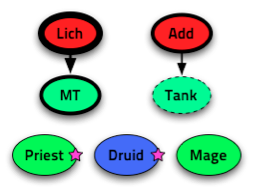
\includegraphics[width=4.7cm]{images/wow_fight1.png} \hspace{1cm} 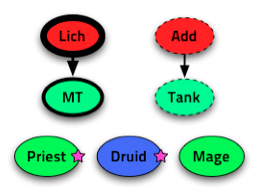
\includegraphics[width=4.7cm]{images/wow_fight2.png}
\caption{Example setup A (left) and B (right), 2 foes, 2 “tanks”, players with stars can heal allies, players with dotted lines will soon die ($ID=true$).}
\label{fig:wow_fight}
\end{center}
\end{figure}

This model has been applied to a simulated situation with 2 foes and 4 allies while our robot took the part of a ``druid'', a versatile class that can cast spells to do direct damages, damages over time, buff (enhancements), debuff, crowd-control, heal and heal over time. We display a schema of this situation in Fig.~\ref{fig:wow_fight} The arrows indicate foes attacks on allies. The larger the ring is, the more health points the characters have. MT stands for ``main tank'', Add for ``additional foe''. We worked with the skills corresponding to a Druid. HOT stands for heal over time, DOT for damage over time, ``abol'' for abolition and ``regen'' for regeneration, a ``buff'' is an enhancement and a ``dd'' is a direct damage. ``Root'' is a spell which disables the target to move for a short period of time, useful to flee or to put some distance between the enemy and the druid to cast attack spells. ``Small'' spells are usually faster to cast than ``big'' spells.

\begin{eqnarray*}
Skills \in \{ small\_heal, big\_heal, HOT, poison\_abol, malediction\_abol,\\
            buff\_armor, regen\_mana, small\_dd, big\_dd, DOT, debuff\_armor, root \}
\end{eqnarray*}

We did not do the ``Identification'' part, which consists in learning the probability tables from observations. To keep things simple and because we wanted to analyze a little the model, we worked with manually defined probability tables. So we introduced ``soft evidences'', indeed parameters that will modify the conditional probability tables, which we will change to watch their effects. For instance the ``soft evidence that a selected target is foe'' and the ``soft evidence that a selected target will soon die ($ID=true$)'' that will consequently modify the probability tables of $P(A_i)$ and $P(ID_i)$ respectively. We set the probability to target the same target as before to 0.4 and the previous target to ``Lich'' so that the prior probability for all other 6 targets is 0.1 (4 times more chances to target the Lich than any other character). We set the soft evidence $P(A_i=false|T=i)$ to 0.6. This means that our robotic druid is mainly a damage dealer and not a healer. For the ``target selection'' model, we can see on Fig.~\ref{fig:wow_target} (left) that the evolution from selecting the main foe ``Lich'' to selecting the ally ``Tank'' is driven by the increase of ``soft evidence that a selected target will soon die'' and our robot eventually moves on targeting his(its) ``Tank'' ally (to heal him). We can see on Fig.~\ref{fig:wow_target} (right) that, at some point, the robotic Druid prefers to kill the dying add to save his ally Tank instead of healing him. Note that there is no variable showing the relation between ``Add'' and ``Tank'' (the first is attacking the second, who is taking damages from the first), but this is under consideration for a future, more complete, model.

\begin{figure}[h!]
\begin{center}
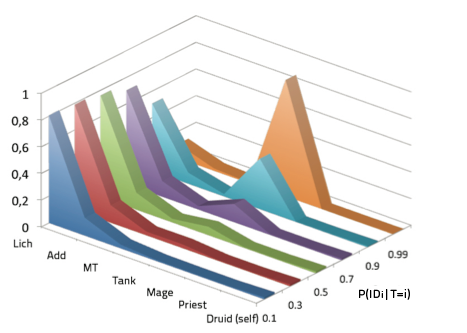
\includegraphics[width=7cm]{images/wow_distrib_target1.png} 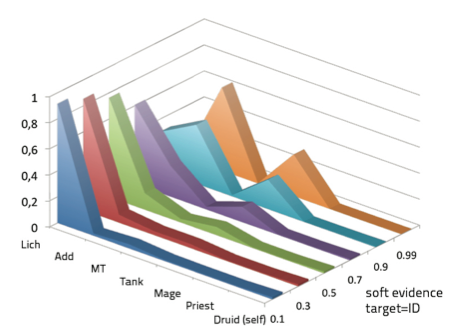
\includegraphics[width=7cm]{images/wow_distrib_target2.png}
\caption{Left: probabilities of targets depending on the soft evidence that a target is dying with setup A. Right: same, with setup B.}
\label{fig:wow_target}
\end{center}
\end{figure}

For the ``skill selection'' model, we can see on Fig.~\ref{fig:wow_skill} the influence of $ID_i$ on Skill which is coherent with the Target distribution: either, in setup A (left), we evolve with the increase of $P(ID_i=true|Target=i)$ to choose to heal our ally or, in setup B (right), to deal direct damage (and hopefully, kill) the foe attacking him. As you can see here, when we have the highest probability to attack the main enemy (``Lich'', when $P(ID_i=true|Target=i)$ is low), who is a $C=tank$, we get a high probability for the Skill $debuff\_armor$. We only cast this skill if the debuff is not already present, so perhaps that we will cast $small\_dd$ instead. To conclude this example, Fig.~\ref{fig:wow_target_skill} shows the distribution on $P(T,S|all\_status\_variables)$ with setup A and the probability to target the previous target (set to ``Lich'' here) only $\approx 2$ times greater than any other character (so that we focus less on the same character), soft evidences $P(ID_i=true|Target=i)=0.9$ and $P(A_i=false|Target=i)=0.6$. In a greedy way, if the first couple $(T,S)$ is already done or not available, we take the second.

\begin{figure}[h!]
\begin{center}
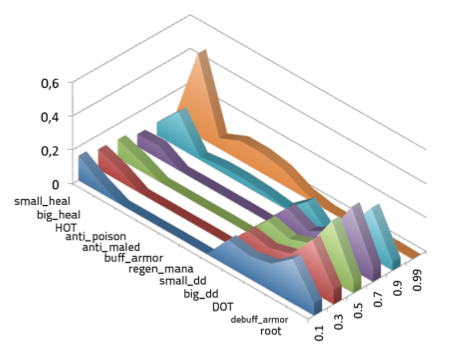
\includegraphics[width=7cm]{images/wow_distrib_skill1.png} 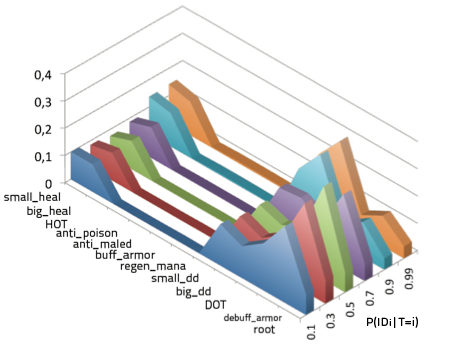
\includegraphics[width=7cm]{images/wow_distrib_skill2.png}
\caption{Left: Probabilities of skills depending on the soft evidence that a target is dying with setup A. Right: same, with setup B.}
\label{fig:wow_skill}
\end{center}
\end{figure}

\begin{figure}[h!]
\begin{center}
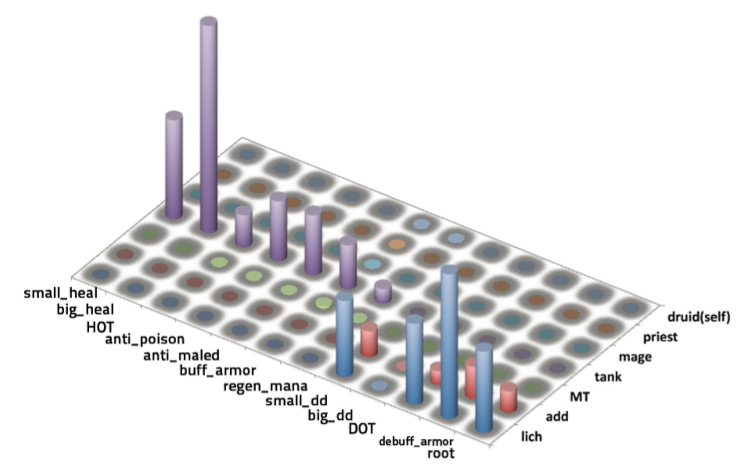
\includegraphics[width=11cm]{images/wow_distrib_target_skill.png}
\caption{Log-probabilities of Target and Skill with setup A, and $P(ID|Target)=0.9, P(A|Target)=0.6$}
\label{fig:wow_target_skill}
\end{center}
\end{figure}

\subsection{Discussion}

This model has to be applied in a real MMORPG, out of its simulated sandbox, to reveal all its shortcomings and be updated. We can already think of some future difficulties, for instance there is a possibility for many games that the Skill variable will be very big and that it will imply a too high computational cost. For that concern, we propose to clusterize the skills in global skills ($GS$) (as it can be seen in the description of the example). This approach to break down the complexity of computation is general and can be used with other variables. The skill variable $S$ can then be the subset of skills corresponding to the clustering of $GS$, for instance we could have:

$$GS \in \{SkillHeal, SkillBuff, SkillAttack, SkillDebuff\}$$
$$S = SkillHeal \in \{skill_1 \dots skill_j\}$$
$$S = SkillBuff \in \{skill_{j+1} \dots skill_k\}$$
$$S = SkillAttack \in \{skill_{k+1} \dots skill_l\}$$
$$S = SkillDebuff \in \{skill_{l+1} \dots skill_m\}$$

Global skills joint distribution: as for the “Skill joint distribution” without Resists. It will take advantage of splitting between allies and foes.

\begin{eqnarray*}
P(GS,T,HP_{1:n},D_{1:n},A_{1:n},\Delta HP_{1:n}, ID_{1:n}, C_{1:n}) = \\
P(GS).P(T).\prod_{i=1}^n [ P(HP_i | A_i, C_i, GS, T).P(D_i | A_i, GS, T).P(A_i | GS, T)\\
                        .P(\Delta HP_i | A_i, GS, T).P(ID_i | GS, T).P(C_i | A_i, GS, T)]
\end{eqnarray*}

Specialized skills joint distribution:

\begin{eqnarray*}
P(S,GS,T,HP_{1:n},D_{1:n},A_{1:n},\Delta HP_{1:n}, ID_{1:n}, C_{1:n}, R_{1:n}) = \\
P(S|GS).P(T).\prod_{i=1}^n [ P(HP_i | A_i, C_i, S, T).P(D_i | A_i, S, T).P(A_i | S, T)\\
                        .P(\Delta HP_i | A_i, S, T).P(R_i | C_i, S, T).P(ID_i | S, T).P(C_i | A_i, S, T)]
\end{eqnarray*}
for the corresponding S. So that we can ask the question:
$$P(S | GS, T, hp_{1:n}, d_{1:n}, a_{1:n}, \Delta hp_{1:n}, id_{1:n}, c_{1:n}, r_{1:n})$$

that will trigger $P(GS|T,\dots)$, itself triggering $P(T|all\_state\_variables)$. Choosing to do with or without the intermediate $GS$ computation, regrouping abilities by types, is mainly a question of computational time.

The choice of the skill or ability to use and the target on which to use it puts hard constraints on every others decisions the autonomous agent has to take to perform its ability action. Thus, such a model shows that:
\begin{itemize}
    \item cooperative behavior is not too hard to incorporate in a decision (instead of being hard-coded),
    \item it can be learned, either from observations of a human player or by reinforcement (exploration),
    \item it is computationally tractable (for use in all games), the inference is just a series of ``probabilistic \textit{if}s'',
\end{itemize}
Moreover, using this model on another agent than the once controlled by the AI can give a prediction on what it will do, resulting in human-like, adaptive, playing style.

We did not kept at the research track of Bayesian modeling MMORPG games due to the difficulty to work on these types of games: the studios have too much to lose to ``farmer'' bots to accept any automated access to the game. Also, there are no sharing format of data (like replays) and the invariants of the game situations are fewer than in RTS games. Finally, RTS games have international AI competitions which were a good motivation to compare our approach with other game AI researchers.
